% Chapter Template

\chapter{La piattaforma ARM embedded} % Main chapter title

\label{Chapter5} % Change X to a consecutive number; for referencing this chapter elsewhere, use \ref{ChapterX}

\lhead{Capitolo 5. \emph{La piattaforma ARM embedded}} % Change X to a consecutive number; this is for the header on each page - perhaps a shortened title

%-------------------------------------------------------------------------------
%	SECTION 1
%-------------------------------------------------------------------------------

\section{Sistema \emph{embedded}}
Un \emph{personal computer} deve saper rispondere a necessità disomogenee:
lo stesso PC potrebbe essere acquistato da alcuni per essere utilizzato come 
\emph{word processor}, da altri come riproduttore multimediale, e da svariate 
ulteriori persone con diversi scopi. Questo rende indispensabile la 
realizzazione di un sistema \emph{general purpose}, ovvero un sistema che possa 
essere riconfigurato velocemente (ad esempio installando del software 
specifico) a seconda della funzione che bisogna svolgere in quel momento.\\
Un sistema \emph{embedded}, invece, è classicamente caratterizzato dall'essere 
un dispositivo 
\emph{special purpose}, ovvero progettato con lo scopo di svolgere un'unica 
funzione. Di conseguenza non è raro che in un sistema \emph{embedded} 
le scelte architetturali e le risorse disponibili siano funzionali
all'applicazione cui è destinato. Rispetto ai sistemi \emph{general purpose}, 
questo generalmente comporta la presenza di architetture differenti, come la 
memoria Harvard e microprocessori RISC anziché CISC, e di hardware 
\emph{custom}, 
alcune volte addirittura progettato \emph{ad hoc} per determinati compiti.
\`E proprio 
merito dell'elevato livello di 
specializzazione che questi sistemi riescono a raggiungere e superare la 
\emph{performance} di uno \emph{general purpose} adibito allo stesso ruolo, pur 
avendo frequenze di clock e complessità\footnote{Intesa come numero di 
transistori.} minori (mediamente di un fattore $10$) oltre che consumi 
nettamente 
inferiori.
Un sistema di questo tipo è ad esempio una centralina di un'automobile: il 
microcontrollore che svolge questo compito deve impiegare tutte le sue risorse 
(memoria, CPU, interfacce I/O) per elaborare i dati che riceve dai sensori e 
agire in conseguenza di determinate evenienze (e.g., se le ruote slittano 
attiva l'ABS). Il sistema in questione sarà programmato in modo da 
svolgere al massimo delle sue capacità queste funzioni, diventando un elemento 
\emph{specializzato} nel suo compito, privo di qualsiasi flessibilità presente 
in un dispositivo \emph{general purpose}.
Altre caratteristiche tipiche dei sistemi \emph{embedded} sono:
\begin{itemize}
\item Costi contenuti
\item Durata commerciale molto estesa
\end{itemize}
Il miglioramento continuo della tecnologia e dei processi produttivi ha 
certamente influenzato i sistemi integrati, avvicinandoli alla controparte 
\emph{general purpose}. Per fare un esempio le \emph{Graphics Processing Unit} 
(GPU), 
che in precedenza avevano il solo 
scopo dell'accelerazione hardware per la grafica ed una programmabilità assai 
limitata, adesso sono facilmente programmabili ed utilizzate per applicazioni 
scientifiche. Anche la notevole spinta del mercato ha 
contribuito alla richiesta sempre maggiore di un ampliamento delle 
funzionalità nei sistemi integrati: basti pensare all'\emph{Internet of 
Things}. \\
Questo è il motivo per cui la definizione di sistema \emph{embedded} è sempre 
più ampia e discussa, e comprende anche sistemi ibridi caratterizzati sia 
dalle peculiarità dei classici sistemi integrati, sia da funzionalità 
\emph{general purpose}, come la piattaforma Banana Pi discussa a seguire.

%-------------------------------------------------------------------------------
%       SECTION 5.2
%-------------------------------------------------------------------------------
\newpage
\section{Il \emph{single-board} computer Banana Pi M1}
\begin{center}
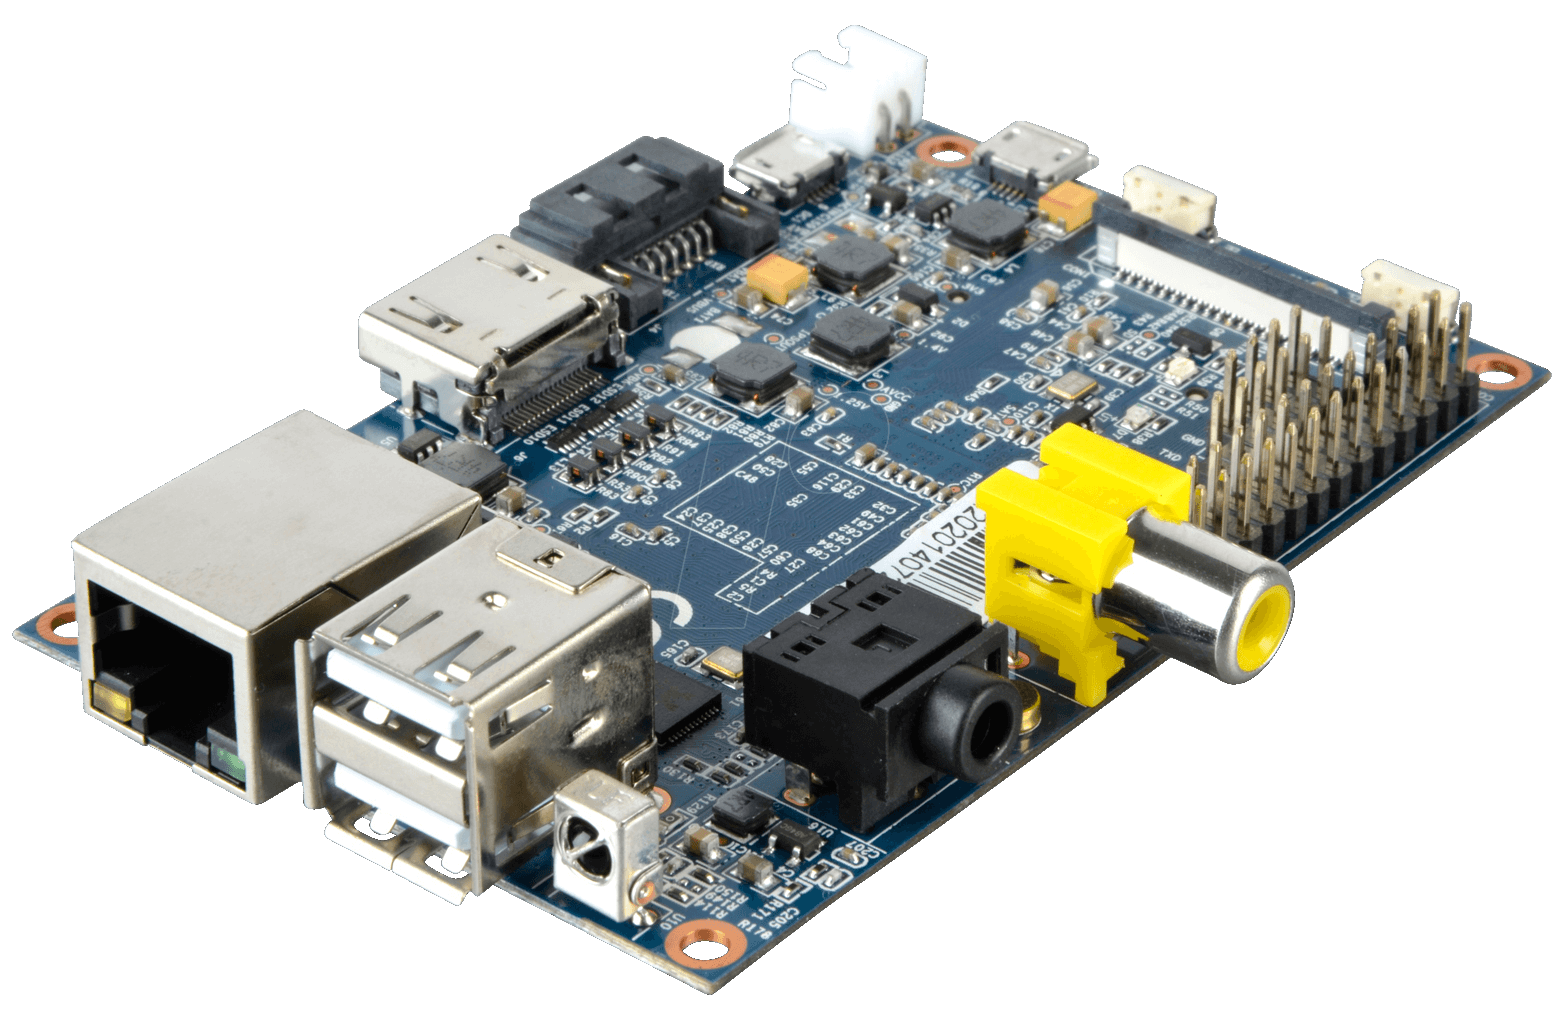
\includegraphics[scale=0.175]{Figures/bananapi.png}\\
\end{center}
Il termine \emph{single-board} viene usato per indicare un'implementazione 
circuitale che sia a tutti gli effetti un computer pur non presentando il 
classico schema con \emph{motherboard}, \emph{daughterboard} e CPU separate in 
diverse schede: un solo circuito stampato contiene tutte e tre.

La nostra \emph{board} di riferimento, il Banana Pi M1 è di questo tipo. Grande 
poco più d'un pacchetto di sigarette, contiene tutto il necessario per 
sopperire a diverse esigenze applicative.

Dotato del \emph{System on a Chip} (SOC) Allwinner A20, dispone di una 
CPU \emph{dual-core} ARM Cortex-A7 con frequenza di 
\textit{clock} pari ad 1GHz ed una GPU
Mediatek Mali-400 MP2 che condividono 1GB di RAM DDR3 di sistema.

Il sistema operativo risiede su \textit{Secure Digital} (SD) \textit{Card}, ma 
le sue capacità di \emph{storage} non sono limitate a quello: ha infatti a 
disposizione un connettore \textit{Serial Advanced Technology Attachment} 
(SATA) affiancato da due pin dedicati all'alimentazione di un'eventuale 
memoria esterna, due porte \textit{Universal Serial Bus} (USB) 2.0 ed una 
Micro-USB con supporto \textit{On-The-Go} (OTG).

Ha a disposizione una porta \textit{High-Definition Multimedia Interface} 
(HDMI) utilizzabile come uscita audio/video ed un connettore video composito, 
oltre alla possibilità di essere collegato ad un pannello \textit{Liquid 
Crystal Display} (LCD) attraverso il connettore \textit{Low-Voltage 
Differential Signaling} (LVDS) presente. Ha anche un collegamento tramite 
\emph{jack} da 3.5 mm utilizzabile come uscita audio ed un microfono integrato 
sulla \emph{board}.

\`E inoltre possibile il collegamento via \textit{Ethernet} grazie alla porta 
\textit{Gigabit} di cui è dotato, dotandolo tra l'altro della possibilità di 
espandere ulteriormente lo spazio di archiviazione normalmente disponibile 
attraverso \emph{network share}.

Possiede infine un connettore \textit{Camera Serial Interface} (CSI) per poter 
essere collegato ad una videocamera digitale, un ricevitore \textit{InfraRed} 
(IR), 26 \textit{pin} \textit{General Purpose Input/Output} (GPIO).

L'alimentazione avviene via Micro-USB, attraverso la porta dedicata.

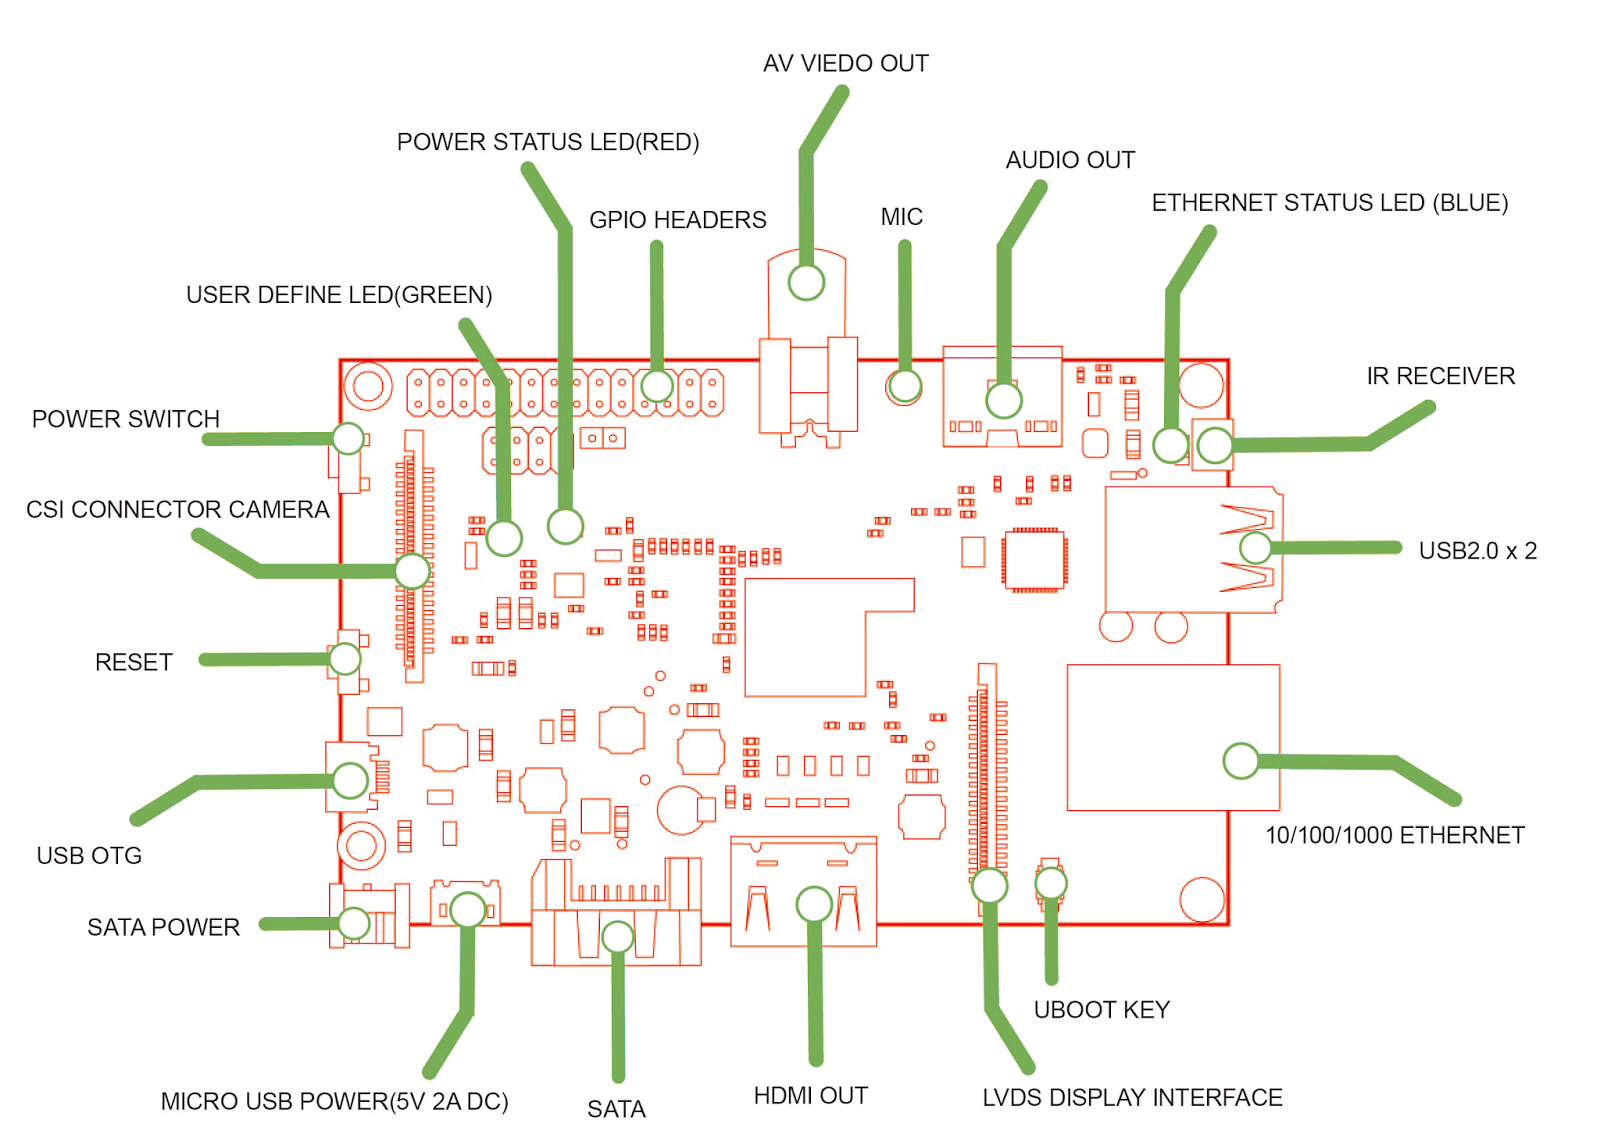
\includegraphics[width=1\textwidth]{Figures/bananapi_schema.png}